\documentclass[10pt]{beamer}

\input{/Users/daniel/Documents/LaTeX/beamer-style.tex}

\title{Maitriser la gestion du code source}
\subtitle{Une brève introduction à \emph{git}}
\date{\today}
\author{Daniel Schreurs}
\institute{Haute École de Province de Liège}
%\titlegraphic{\hfill\includegraphics[height=1.5cm]{logo.eps}}

\setbeamertemplate{frame footer}{\insertsectionhead}
\begin{document}
\maketitle

\setbeamerfont{subsection in toc}{size=\small}
\setbeamerfont{subsubsection in toc}{size=\normalsize}
\setbeamertemplate{section in toc}[sections numbered]
\setbeamertemplate{subsection in toc}[subsections numbered]
\setbeamertemplate{subsubsection in toc}[subsubsections numbered]
\begin{frame}[allowframebreaks]{Table des matières du chapitre}
    \tableofcontents[subsectionstyle=show/show/hide,subsubsectionstyle=show/show/hide,]
\end{frame}

\section{Objectifs}

\begin{frame}{\secname}
    \centerline{
\includegraphics[width=\textwidth]{img/bd1.jpeg}}
\end{frame}

\begin{frame}{\secname}
    \begin{itemize}
        \item Gérer le code source;
        \item Ne plus perdre du code;
        \item Conserver tout l’historique;
        \item Comparer les différentes versions d’un projet;
        \item Garder une trace des personnes intervenant sur le code;
        \item En local ... et sur le cloud\footnote{Par exemple avec GitHub.};
        \item Un standard dans l’ingénierie logiciel.
    \end{itemize}
\end{frame}



\section{Ressources}
\subsection{Quelques liens}
\begin{frame}{\subsecname}
    \begin{itemize}
        \item \href{https://git-scm.com/about}{Documentation officielle};
        \item \href{https://rogerdudler.github.io/git-guide/index.fr.html}{git - petit guide};
        \item \href{https://gitmoji.dev}{gitmoji};
        \item \href{https://cli.github.com}{GitHub CLI brings GitHub to your terminal.};
    \end{itemize}
\end{frame}
\subsection{Quelques livres}
\begin{frame}{\subsecname}
    \centerline{
\includegraphics[height=0.8\textheight]{img/David-Demaree-GIT-FOR-HUMANS.jpg}}
\end{frame}


\begin{frame}{\subsecname}
    \centerline{
\includegraphics[height=0.8\textheight]{img/Version Control with Git.jpg}}
\end{frame}


\begin{frame}{\subsecname}
    \centerline{
\includegraphics[height=0.8\textheight]{img/git pro.jpg}}
\end{frame}


\subsection{GitHub Student Developer Pack}
\begin{frame}{\subsecname}
    \begin{enumerate}
        \item Créer un compte sur \href{https://github.com/join}{GitHub} en renseignant votre adresse étudiant;
        \item Demandez votre \href{https://education.github.com/pack}{pack étudiant}\footnote{Cela vous donne accèes à des logiciels gratuitement ainsi qu'un compte pro}.
    \end{enumerate}

\end{frame}


\section{GitHub}
\begin{frame}{\secname}
    \begin{center}
        \href{https://www.youtube.com/watch?v=w3jLJU7DT5E}{What is GitHub?}
    \end{center}
\end{frame}

\begin{frame}{\secname}
    \begin{itemize}
        \item Plateforme en ligne pour déposer du code\footnote{Avec une visibilité publique ou privée.};
        \item Permettre la collaboration\footnote{La plupart des projets \emph{open source} s’y trouvent. \href{https://github.com/android}{Android}, \href{https://github.com/chromium/chromium}{Chromium}, \href{https://github.com/facebook/react}{React}, \href{https://github.com/flutter/flutter}{flutter}, etcs.};
        \item Se faire une réputation;
        \item Le fichier \lstinline[language=git]!readme.md!\footnote{Un fichier texte au format \href{https://fr.wikipedia.org/wiki/Markdown}{Markdown} éditable avec \href{https://typora.io}{Typora}, \href{https://draftin.com}{Draft}, \href{https://code.visualstudio.com}{Visual Studio Code}, etc.} permet de documenter le dépôt.
    \end{itemize}
\end{frame}

\section{Git}
\subsection{Installation MacOS}

\begin{frame}{\secname : \subsecname}
    \begin{itemize}
        \item Ouvrez l'application \emph{Terminal};
        \item Installer Xcode Command Line Tools avec la commande \lstinline[language=sql]!xcode-select --install!
    \end{itemize}
\end{frame}

\subsection{Installation Windows}
\begin{frame}{\secname : \subsecname}
    \begin{itemize}
        \item Rendez-vous sur \href{https://git-scm.com/downloads}{la page officielle de git};
        \item Télécharger et installer la denière version pour Windows!
        \item Lors de l'installation activez l'utilitaire \emph{git bash}!\footnote{C'est à partir de là que nous exécuterons nos premières commandes.}
    \end{itemize}
\end{frame}
\begin{frame}{\secname : \subsecname}
    \centerline{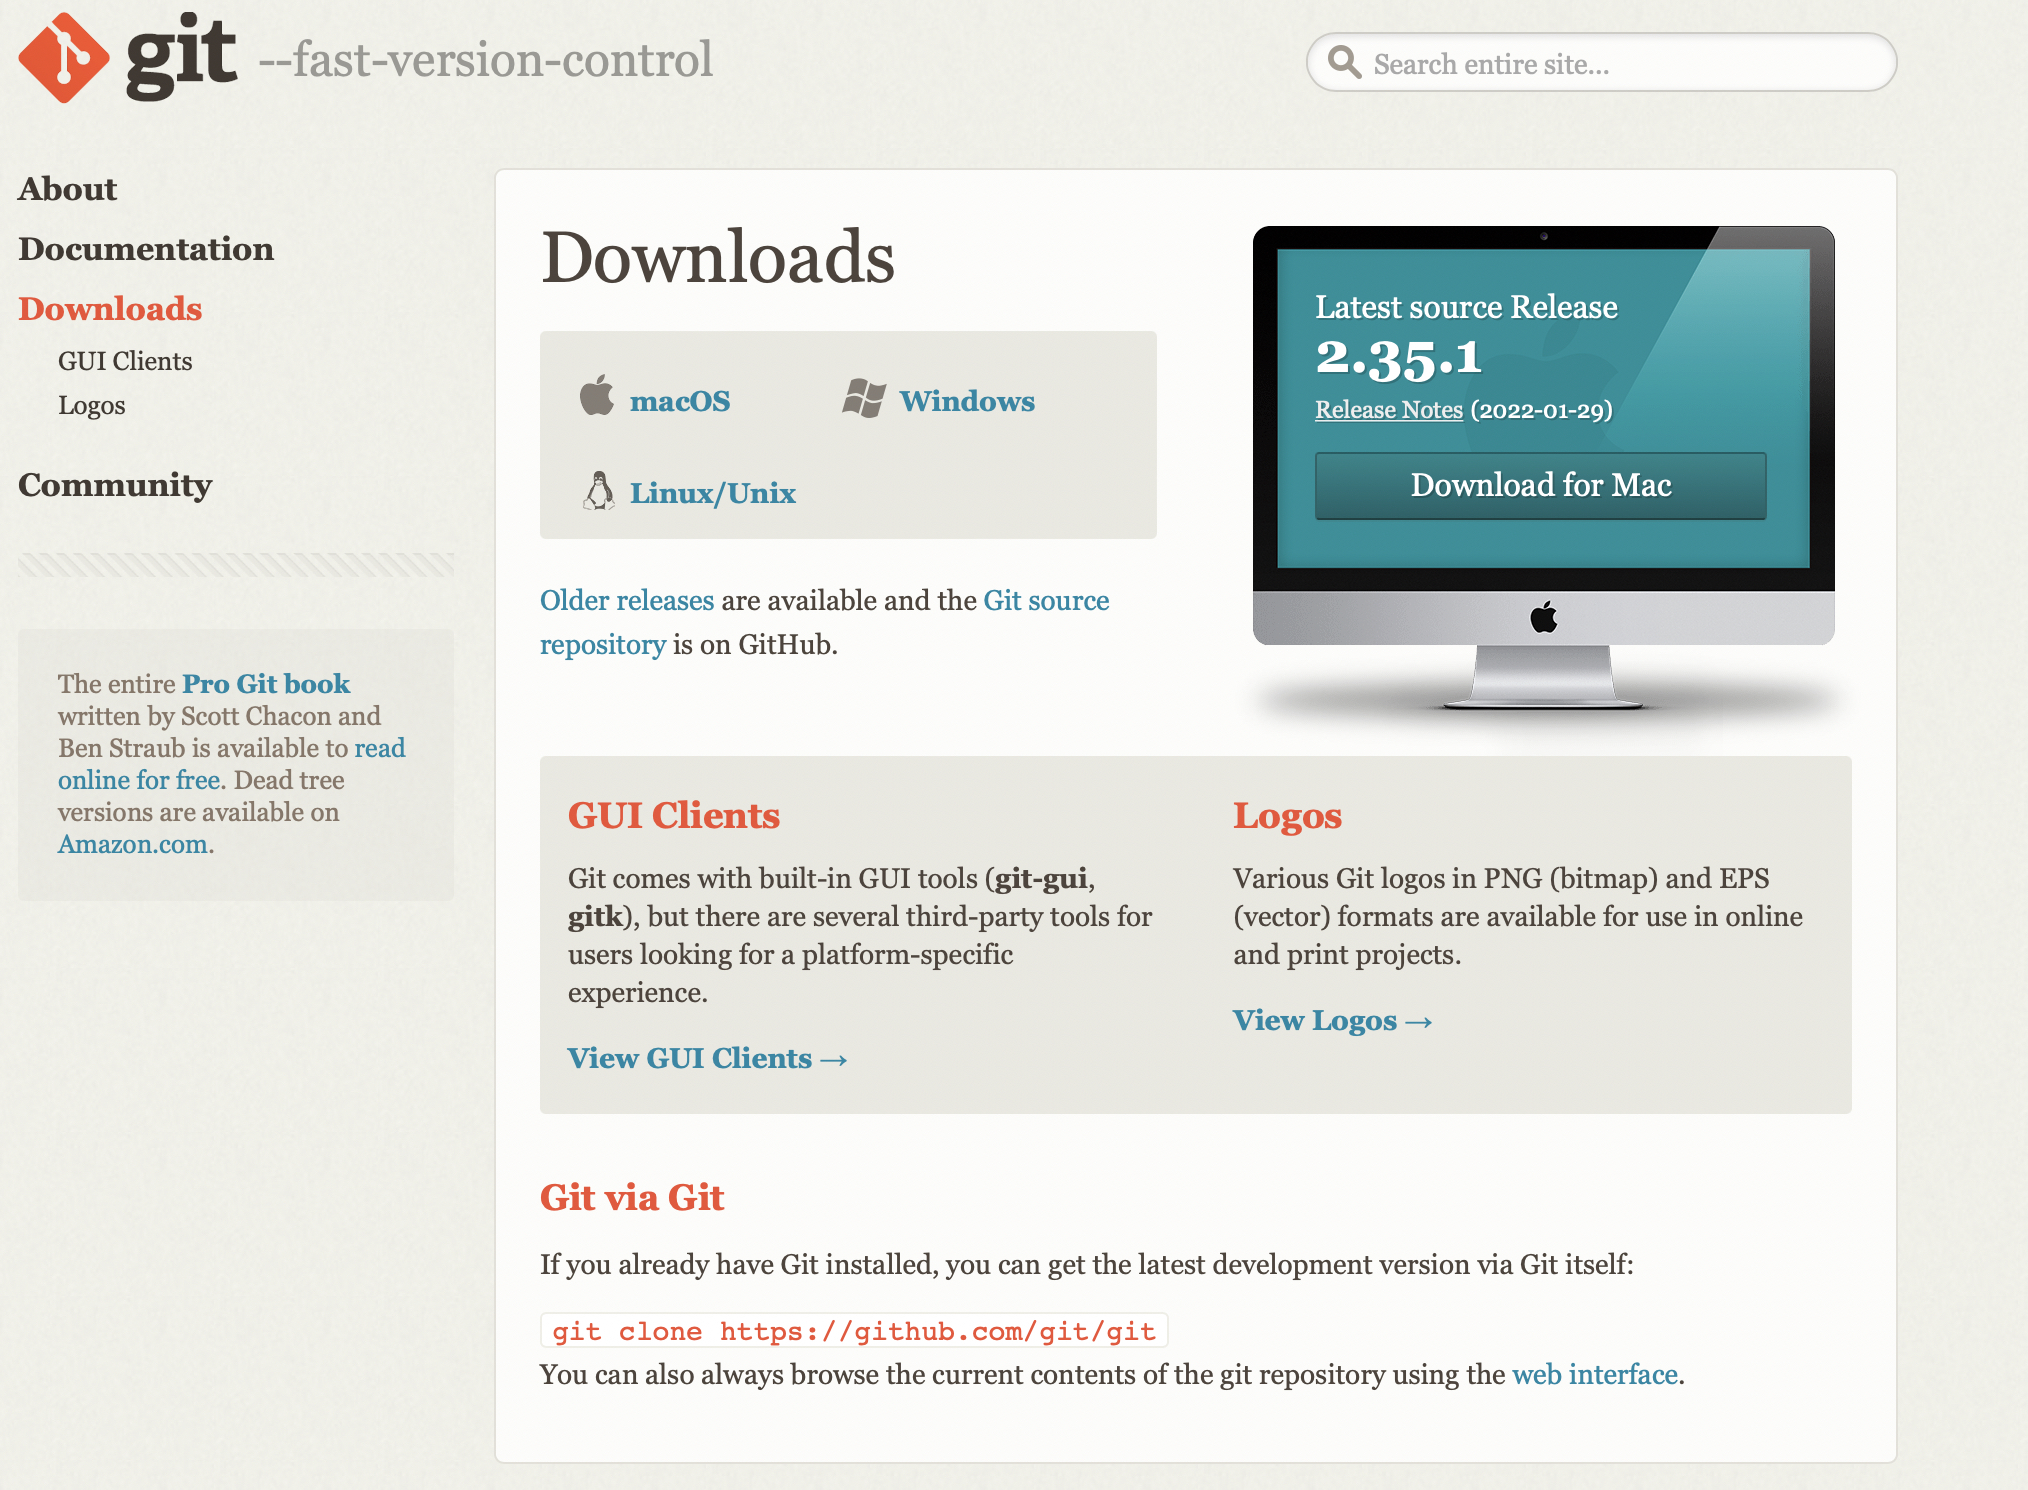
\includegraphics[height=0.8\textheight]{img/git.jpg}}
\end{frame}
\begin{frame}{\secname}
    \begin{itemize}
        \item Télécharger et installer un outil pour gérer en local :
              \href{https://desktop.github.com}{GitHub Desktop} ou \href{https://www.gitkraken.com}{GitKraken} ou \href{https://www.sourcetreeapp.com}{Sourcetree} ou \href{https://www.git-tower.com/mac}{Tower};
        \item Avancer pas à pas en augmentant la difficulté dès que les choses simples sont maîtrisées.
    \end{itemize}
\end{frame}

\section{Démonstration 1}
\begin{frame}{\secname}
    \begin{itemize}
        \item Initialiser un projet;
        \item Document \emph{markdown};
        \item Ajouter des fichiers;
        \item Ajouter le \lstinline[language=git]!.gitignore!;
        \item Publier les changements.
    \end{itemize}
\end{frame}

\section{gitignore}
\begin{frame}{\secname}
    \begin{itemize}
        \item Créer un fichier \lstinline[language=c]!.gitignore! à la racine du répertoire à gérer;
        \item Ce fichier peut être créé automatiquement et simplement à partir du site \href{https://www.gitignore.io/}{gitignore.io}. Encodez par exemple les mots-clés "CSharp", "Windows", etc.
        \item Objectif : dans la gestion des sources, on ne garde que ce qui est important. Par exemple, les fichiers .exe ne sont pas enregistrés. Puisqu’ils dépendent de l’environnent.
    \end{itemize}
\end{frame}

\section{Commandes}
\subsection{Créer un nouveau dépôt}
\begin{frame}{\secname : \subsecname}
    \begin{itemize}
        \item Créez un nouveau dossier vide;
        \item Lancez un terminal dans ce dossier;
        \item Initialisez un dépôt avec la commande :
              \lstinline[language=git]!git init!
    \end{itemize}
\end{frame}

\subsection{Cloner un dépôt}
\begin{frame}{\secname : \subsecname}
    \begin{itemize}
        \item Créez une copie de votre dépôt local en exécutant la commande :
              \lstinline[language=git]!git clone /path/to/repository!
        \item Si vous utilisez un serveur distant, cette commande sera
              \lstinline[language=git]!git clone username@host:/path/to/repository!
    \end{itemize}
    \centerline{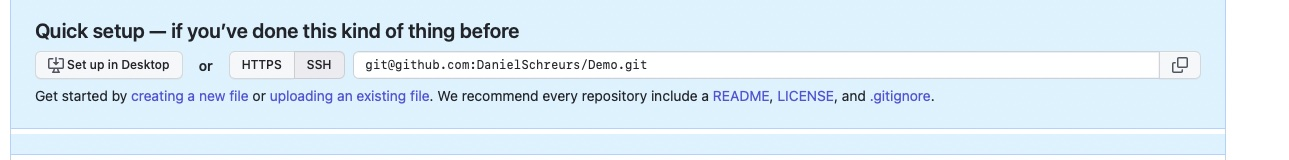
\includegraphics[width=\textwidth]{img/GitHUbClone.jpg}}
\end{frame}

\subsection{Communiquer avec le serveur GitHub}
\begin{frame}{\secname : \subsecname}
    Première interaction avec GitHub depuis le terminal :
    \begin{itemize}
        \item Vous devez renseigner votre identifiant et MDP GitHub;\footnote{Ou renseigner une paire de clés SSH en suivant \href{https://docs.github.com/en/authentication/connecting-to-github-with-ssh}{ce tutoriel}.}.
        \item Vous devez renseigner un username et une adresse mail.\footnote{C’est juste un label. Vous êtes libre de choisir l’adresse mail.}
    \end{itemize}
\end{frame}

% \subsection{Arbres}
% \begin{frame}{\secname : \subsecname}
%     Votre dépôt local est composé de trois \emph{arbres} gérés par git.
%     \begin{itemize}
%         \item Votre \emph{espace de travail} qui contient vos fichiers.
%         \item Un \emph{Index} qui joue un rôle d'espace de transit;
%         \item Le HEAD qui pointe vers la dernière validation que vous ayez faite.
%     \end{itemize}
% \end{frame}


\subsection{Ajouter \& valider}
\begin{frame}{\secname : \subsecname}
    \begin{itemize}
        \item Vous pouvez proposer un changement (l'ajouter à l'Index) en exécutant les commandes
              \lstinline[language=git]!git add <filename>! ou
              \lstinline[language=git]!git add .!\footnote{Attention, dans ce cas il est primordial d'avoir un fichier .gitignore à la racine du dépôt.}
        \item Pour valider ces changements, utilisez
              \lstinline[language=git]!git commit -m "Message de validation"!
    \end{itemize}
\end{frame}

\subsection{Envoyer des changements}
\begin{frame}{\secname : \subsecname}
    \begin{itemize}
        \item Pour les envoyer sur votre dépôt distant, exécutez la commande
              \lstinline[language=git]!git push origin main!\footnote{Remplacez main par la branche dans laquelle vous souhaitez envoyer vos changements. }
        \item Si vous n'avez pas cloné votre dépôt existant, vous devez l'ajouter avec
              \lstinline[language=git]!git remote add origin <server>!\footnote{Maintenant, vous pouvez envoyer vos changements vers le serveur distant sélectionné}
    \end{itemize}
\end{frame}

\subsection{Branches}
\begin{frame}{\secname : \subsecname}
    Les branches sont utilisées pour développer des fonctionnalités isolées des autres.
    \begin{itemize}
        \item   Créer une nouvelle branche nommée $feature\_x$ et passer dessus pour l'utiliser
              \lstinline[language=git]!git checkout -b feature_x!
        \item Retourner sur la branche principale
              \lstinline[language=git]!git checkout main!
        \item Et supprimer la branche
              \lstinline[language=git]!git branch -d feature_x!
    \end{itemize}
    \metroset{block=fill}
    \begin{alertblock}{Important}
        Une branche n'est pas disponible pour les autres tant que vous ne l'aurez pas publiée sur le dépôt distant.
        \lstinline[language=git]!git push origin <branch>!
    \end{alertblock}
\end{frame}


\begin{frame}{\secname : \subsecname}
    \metroset{block=fill}
    \begin{alertblock}{Important}
        Historiquement, la banche s’appelait \emph{Master}. Maintenant on préconise de l’appeler \emph{Main}. Soyez vigilant.
        \href{https://stackoverflow.com/questions/64249491/difference-between-main-branch-and-master-branch-in-github}{Difference Between Main Branch and Master Branch in GitHub?}
    \end{alertblock}
\end{frame}

\subsection{Mettre à jour \& fusionner}
\begin{frame}{\secname : \subsecname}

    \begin{itemize}
        \item Mettre à jour le dépôt local \lstinline[language=git]!git pull!
        \item Fusionner une autre branche avec la branche activ \lstinline[language=git]!git merge <branch>!
        \item Malheureusement, ça n'est pas toujours possible...Vous devez alors régler les conflits;
        \item Après l'avoir fait, vous devez les marquer comme fusionnés avec \lstinline[language=git]!git add <filename>!;
        \item Vous pouvez en avoir un aperçu en utilisant \lstinline[language=git]!git diff <source_branch> <target_branch>!.
    \end{itemize}
\end{frame}

\subsection{Remplacer les changements locaux}
\begin{frame}{\secname : \subsecname}
    \begin{itemize}
        \item Annuler les changements locaux en utilisant cette commande \lstinline[language=git]!git checkout -- <filename>!\footnote{Cela remplacera les changements avec le dernier contenu du HEAD.}
        \item Récupérez le dernier historique depuis le serveur et pointez la branche principale locale dessus comme ceci \lstinline[language=git]!git fetch origin!
    \end{itemize}
\end{frame}

\subsection{Pull Requests}
\begin{frame}{\secname : \subsecname}
    \centerline{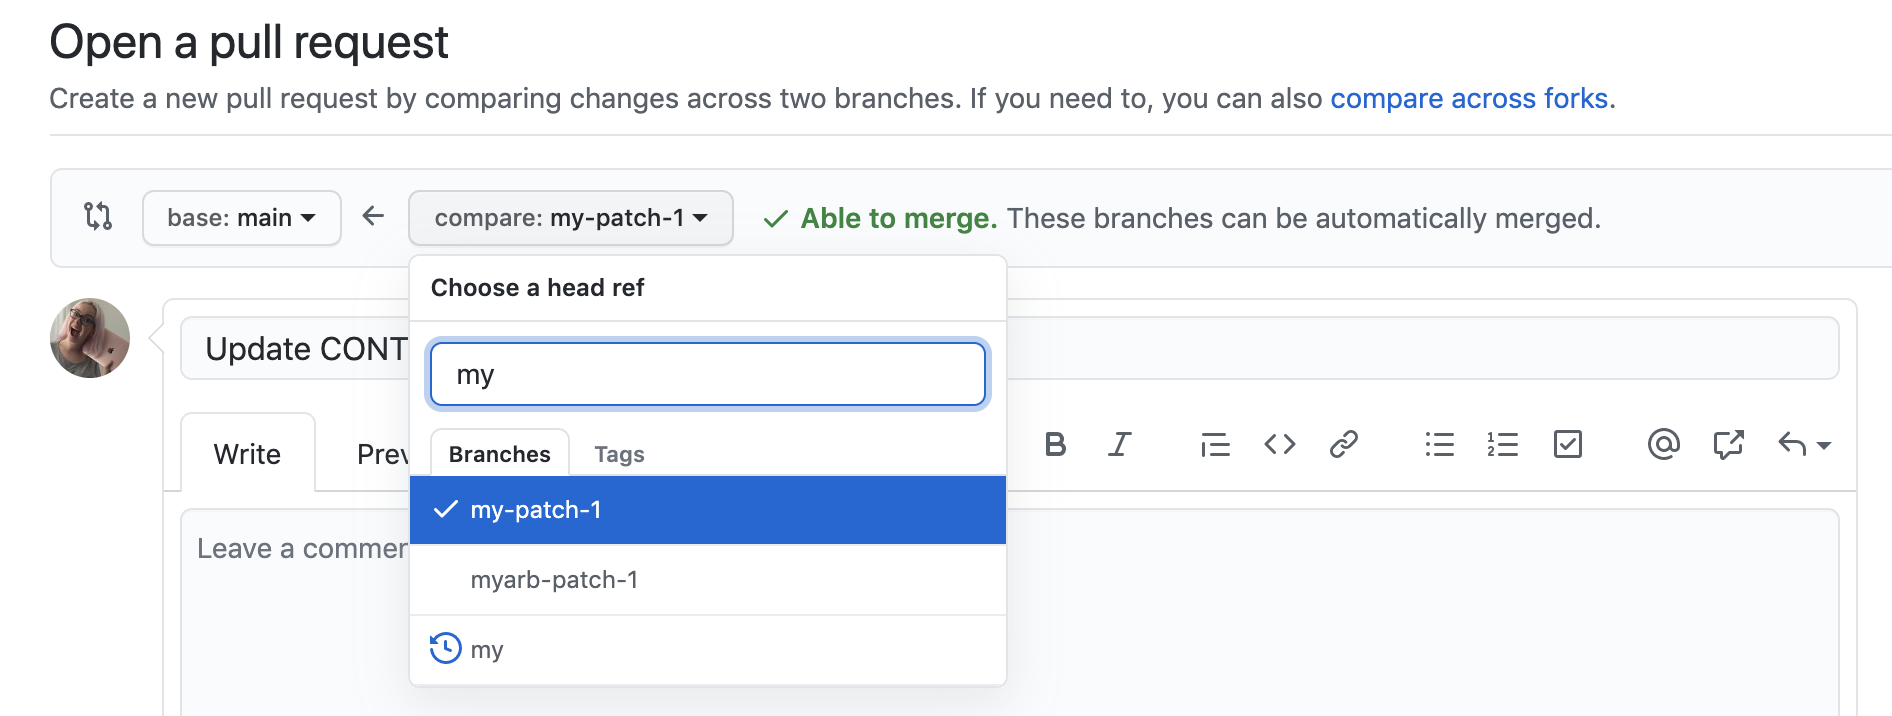
\includegraphics[width=\textwidth]{img/pull-request-review-edit-branch.png}}
\end{frame}

\begin{frame}{\secname : \subsecname}
    \begin{itemize}
        \item Proposition de changement de code.
        \item Soumission de modifications au projet.
        \item Favorise la collaboration.
        \item Révision et discussion des modifications.
        \item Garantit la qualité du code via des vérifications.
    \end{itemize}
\end{frame}



\section{Synthèse des commandes}
\begin{frame}{\secname}
    \centerline{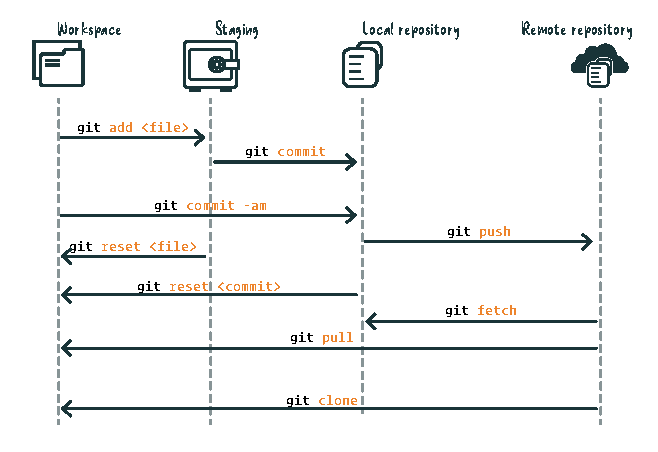
\includegraphics[height=0.8\textheight]{img/synthese.eps}}
\end{frame}


\section{Démonstration 2}
\begin{frame}{\secname}
    \begin{itemize}
        \item Accepter un devoir (GitHub Classroom);
        \item \emph{Cloner} un projet;
        \item Ajouter et modifier des fichiers C\#;
        \item Publier les changements;
        \item Créer une branche;
        \item Ajouter des changements;
        \item Publier la branche avec ses changements;
        \item Fusionner la branche dans \emph{main}.
    \end{itemize}
\end{frame}

\appendix

\begin{frame}[standout]
    That's All Folks!
\end{frame}

\begin{frame}{}
    \centerline{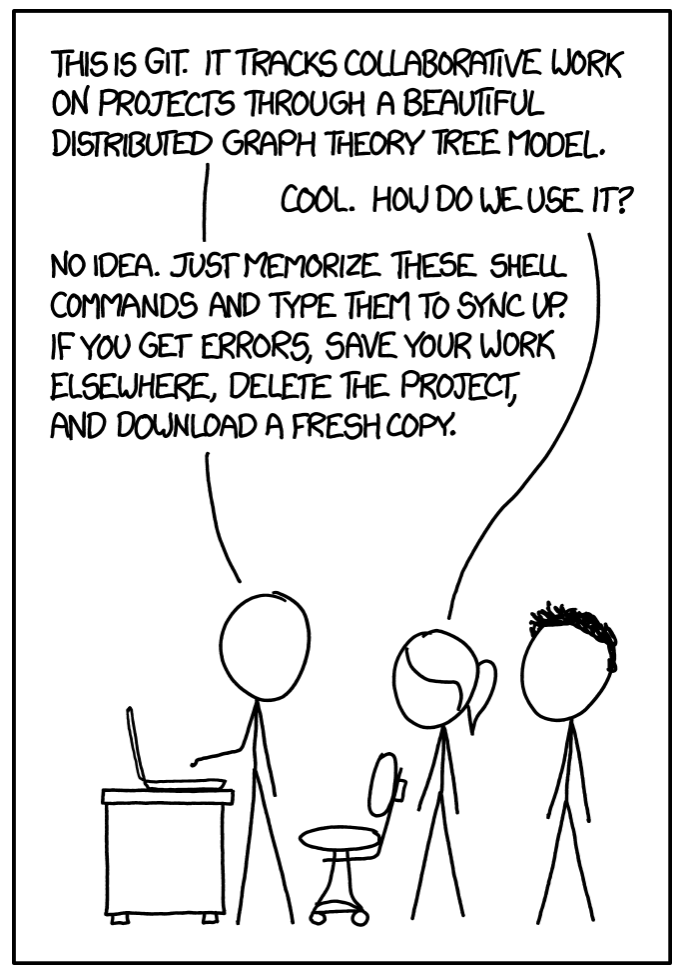
\includegraphics[height=0.9\textheight]{img/bd2.png}}
\end{frame}

\end{document}
